  %%%%%%%%%%%%%%%%%%%%%%%%%%%%%%%%%%%%%%% -*- coding: utf-8; mode: latex -*- %%
  %
%%%%%                       CHAPTER
 %%%
  %

% $Id: 3100-nihil-molestiae.tex,v 1.1 2007/11/23 09:52:43 david Exp $
% $Log: 3100-nihil-molestiae.tex,v $
% Revision 1.1  2007/11/23 09:52:43  david
% *** empty log message ***
%
%

  %%%%%%%%%%%%%%%%%%%%%%%%%%%%%%%%%%%%%%%%%%%%%%%%%%%%%%%%%%%%%%%%%%%%%%%%%%%%%
  %
%%%%%                    HEAD MATTER
 %%%
  %

\chapter{Solution}
The solution we propose to improve the throughput can be summarized as \textit{Optimistic Concurrency Control with Snapshot Isolation on Semantic Related Group}. The solution algorithm consists of the following four phases:
\begin{enumerate}[noitemsep]
	\item \textbf{Read Phase}: resolving the semantic related group and cache the snapshot copy within the handling transaction.
	\item \textbf{Execution Phase}: transaction read/write operations are performed on its own snapshot and never fetch data from database.
	\item \textbf{Validation Phase}: snapshot's related data rows are fetched from the database. If their versions all match with the snapshot copy, go to update phase; else, abort and retry current transaction.
	\item \textbf{Update Phase}: update related data in the database table. Abort and retry transactions if the instance already exists in the database for "new" data. For successful updates, the versions of the modified rows will be increased by 1.
\end{enumerate}
\label{ch:Design}

\noindent The phases mentioned above will be illustrated in the following sections with more details. The complete algorithm pseudocode can be found in Algorithm~\ref{algo:pseudocode}.
\section{Resolving the Semantic Related Group}

Resolving the semantic related group for each transaction is the fundamental step to preclude \textit{anomalies} in our implementation. The \textit{constraint violation}~\cite{berenson1995critique} between individual data is formed within a semantic related group. In Hop-HDFS, each metadata operation is implemented as a single transaction running by a worker thread. Any metadata operation related to the namespace will have one or two input parameters, called \textit{Path}. Here's two examples for operation methods in the Filesystem API:

\begin{itemize}[noitemsep]
	\item boolean \textbf{mkdirs} (Path \textit{f}): \textit{f} is the path of the INodeDirectory to be created
	\item boolean \textbf{rename} (Path \textit{src}, Path \textit{dst}): \textit{src} is the path to be renamed, \textit{dst} is the new path after rename
\end{itemize} 

\noindent Each \textit{Path} object is related to a string representation of the "/" based absolute path name. For example, in Figure~\ref{fig:hoptree}, the path for INode \textit{h} is: 
\begin{center}
	/a/d/f/h
\end{center}

\noindent Therefore, with the preservation of the \textit{directed tree structure}, we can resolve a semantic related group for each INode along the edge of ancestors into a LinkedList. The semantic related group representation for INode \textit{h} is:
\begin{center}
	h: \{/-$>$a-$>$d-$>$f\}
\end{center}

\noindent In other words, when mutating INode \textit{h}, all the semantic constraint can be found within INodes \textit{/, a, d, f}. With this knowledge, we can maintain the strong consistency semantics in original HDFS.

\noindent For each row in \textit{inodes table}, the $<$name, parent\_id$>$ pair is the \textit{Primary Key}. With the full path string, we can iteratively resolve its semantic related rows by primary key lookups directly from database as shown in Table~\ref{table:semanticrelatedTable}.

\begin{table}[h]
	\centering
	\begin{tabular}{|c|c|c|c|c|}
		\hline
		~ & \textbf{id} & \textbf{parent\_id} & \textbf{name} & \textbf{other parameters...} \\ \hline
		Related * & 1 & 0 & / & ... \\ \hline
		Related * & 2 & 1 & a & ... \\ \hline
		~ & 3 & 1 & b & ... \\ \hline
		~ & 4 & 1 & c & ... \\ \hline
		Related * & 5 & 2 & d & ... \\ \hline
		~ & 6 & 3 & e & ... \\ \hline
		Related * & 7 & 5 & f & ... \\ \hline
		~ & 8 & 6 & g & ... \\ \hline
		Selected \checkmark & 9 & 7 & h & ... \\ \hline
		~ & 10 & 7 & i & ... \\ \hline
	\end{tabular}
	\caption{Table Representation for the Semantic Related Group}
	\label{table:semanticrelatedTable}
\end{table}
  %%%%%%%%%%%%%%%%%%%%%%%%%%%%%%%%%%%%%%%%%%%%%%%%%%%%%%%%%%%%%%%%%%%%%%%%%%%%%
  %
%%%%%                      SECOND SECTION
 %%%
  %

\section{Per-Transaction Snapshot Isolation}

As we mentioned before, MySQL Cluster supports only the READ COMMITTED transaction isolation level, which means that the committed results of write operations in transactions will be exposed by reads in other transactions. Within a long running transaction, it could read two different versions of data, known as \textit{fuzzy read}, and it could also get two different sets of results if the same query is issued twice, known as \textit{phantom read}.

\noindent \textit{Snapshot isolation} guarantees that all reads made within a transaction see a consistent view of at the database. At the beginning of the transaction, it reads data from a snapshot of the latest committed value. During transaction execution, reads and writes are performed on the this snapshot.

\noindent In commercial database management systems, like Microsoft SQL Server, Oracle, etc, \textit{snapshot isolation} is implemented within multi version concurrency control (MVCC)~\cite{berenson1995critique} on database server side. However, we need to implement snapshot isolation on the application side since MySQL Cluster supports only the READ COMMITTED isolation level.

\noindent After resolving the semantic related group, we take a snapshot on selected rows as well as all related rows of the committed values from database. This snapshot will be cached in-memory within its transaction. Each transaction will have its own copy of snapshot during the lifetime. All transaction operations will be performed on its own snapshot. Therefore, we called it Per-Transaction Snapshot Isolation.

\subsection{Fuzzy Read and Phantom Read are Precluded}

\noindent Before validation phase, the transaction will never fetch any data from database since it has all the semantic related rows in the cached snapshot. Therefore, the snapshot provides a consistent view of data for each transaction from read phase until validation phase. Hence: 
\begin{itemize}[noitemsep]
	\item \textit{Fuzzy Read} is precluded by \textit{snapshot isolation}: As we can see from Figure~\ref{fig:snapfuzzy}, the second read of Transaction 1 read from snapshot instead of database, not affected by the value committed by Transaction 2.
	
	\item \textit{Phantom Read} is also precluded by \textit{snapshot isolation on Semantic Related Group}: As we can see from Figure~\ref{fig:snapphantom}, Transaction 1 snapshot the semantic related group of x after the first count operation. So its second count operation is not affected by the value inserted by Transaction 2 since it counts from the snapshot.
	
\end{itemize} 

\begin{figure}[!h]
	\centering
	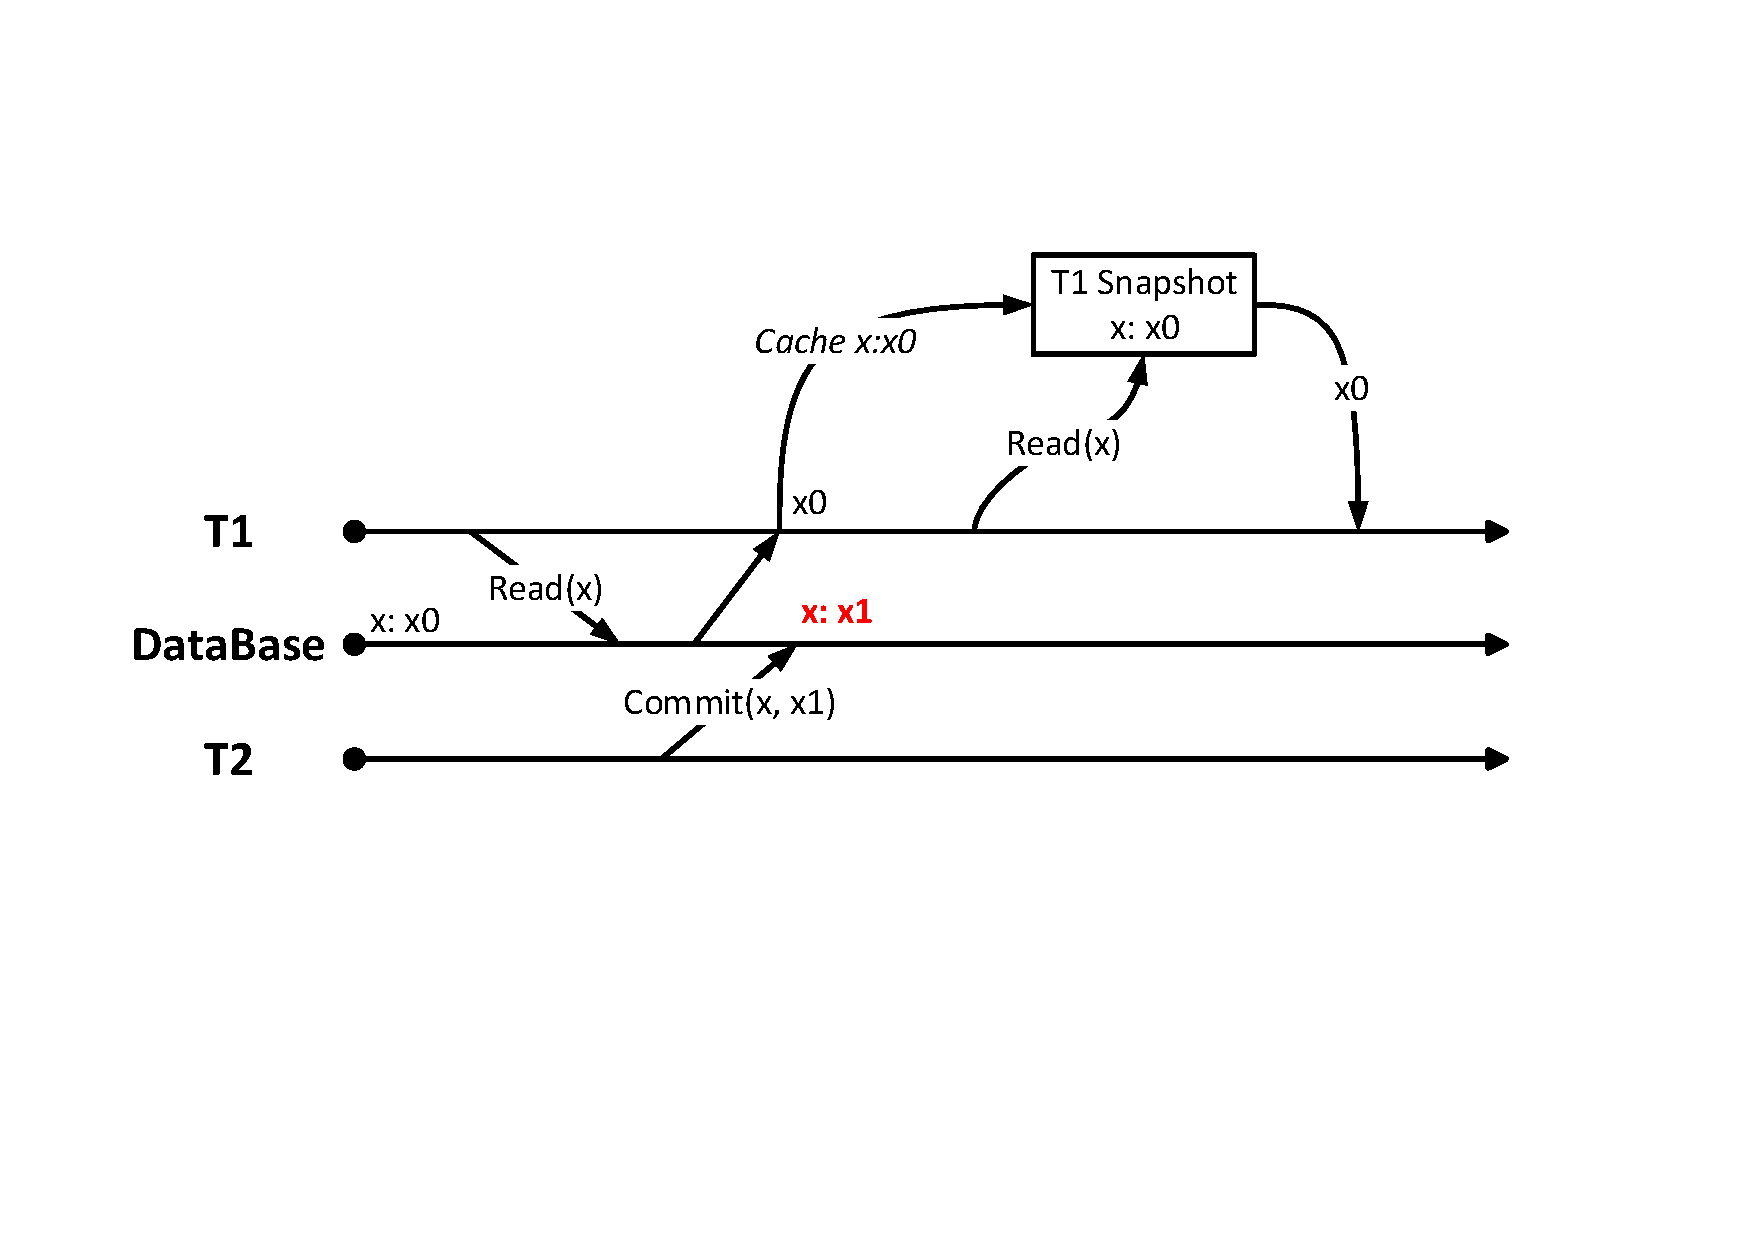
\includegraphics[width=\linewidth]{figs/snapfuzzy.pdf}
	\caption{Snapshot Isolation Precludes Fuzzy Read}
	\label{fig:snapfuzzy}
\end{figure}

\begin{figure}[!h]
	\centering
	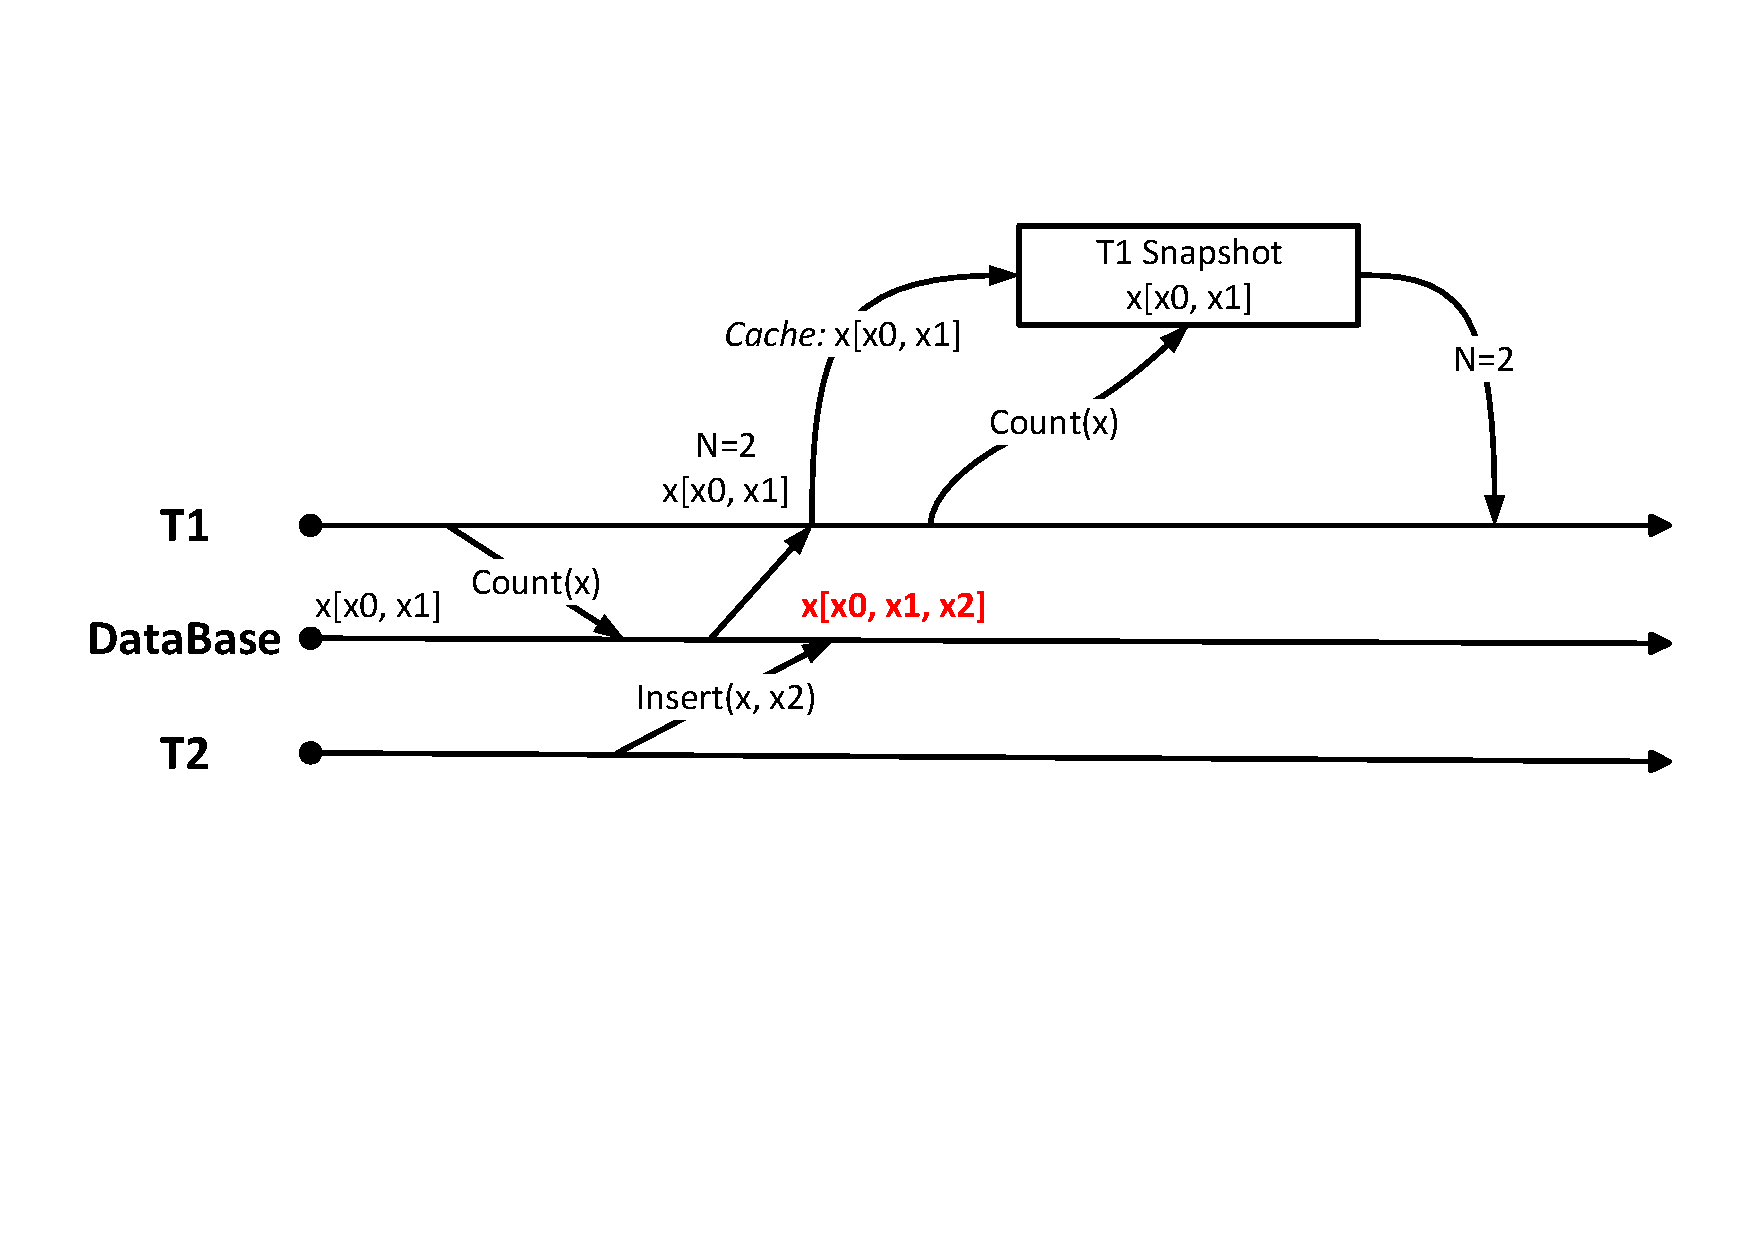
\includegraphics[width=\linewidth]{figs/snapphantom.pdf}
	\caption{Snapshot Isolation with Semantic Related Group Precludes Phantom Read}
	\label{fig:snapphantom}
\end{figure}
  %%%%%%%%%%%%%%%%%%%%%%%%%%%%%%%%%%%%%%%%%%%%%%%%%%%%%%%%%%%%%%%%%%%%%%%%%%%%%
  %
%%%%%                         ANOTHER SECTION
 %%%
  %
  
\section{ClusterJ and Lock Mode in MySQL Cluster}

\textit{ClusterJ}~\cite{mysqlclusterj} is a Java connector based on object-relational mapping persistence frameworks to access data in MySQL Cluster. Since it uses a JNI bridge to the NDB API for direct access to NDB Cluster, it doesn't depend on the MySQL Server to access data in MySQL Cluster, which means that ClusterJ can perform some operations much more quickly since it communicates to the data nodes directly. 

\noindent Therefore, with the mapping from java classes to database tables, we use ClusterJ to fetch and persist data in MySQL Cluster using primary key and unique key operations for single-table queries (not supporting multi-table operations though). If we recall the architecture of MySQL Cluster from Figure~\ref{fig:mysqlclusterarchitecture}, ClusterJ will be the Java Persistence API between Hop-HDFS and the \textit{Data Nodes} (ndbd) , without going through \textit{MySQL Servers} (mysqld).

\noindent Unlike \textit{Two-Phase Locking} (2PL), there are three lock modes in MySQL Cluster:

\begin{enumerate}[noitemsep]
	\item \textbf{SHARED} (Read Lock, RL): Set a shared lock on rows
	\item \textbf{EXCLUSIVE} (Write Lock, WL): Set an exclusive lock on rows
	\item \textbf{READ\_COMMITTED} (Read Committed, RC): Set no locks but read the most recent committed values
\end{enumerate}

\noindent \textit{Shared} and \textit{Exclusive} locks have the same definition of those in Two-phase Locking. For \textit{Read\_Committed}, it is implemented for consistent nonlocking reads, which means that a fresh committed snapshot of data row is always presented to a query of database, regardless of whether Shared Lock or Exclusive Lock are taken on the current row or not. It is based on \textit{Multiversion Concurrency Control} described by Oracle~\cite{oraclemvcc} for read consistency from a single point in time (\textit{statement-level read consistency}). See Table~\ref{table:locktable} for the reference of the blocking effect.

\noindent We use \textit{Read\_Committed} for the \textit{read phase} in our algorithm.

\begin{table}[h]
	\centering
	\begin{tabular}{|c|c|c|c|}
		\hline
		\textbf{Lock Type} & \textbf{SHARED} & \textbf{EXCLUSIVE} & \textbf{READ\_COMMITTED} \\ \hline
		SHARED             & \checkmark               & Block              & \checkmark                        \\ \hline
		EXCLUSIVE          & Block           & Block              & \checkmark                        \\ \hline
		READ\_COMMITTED    & \checkmark               &            \checkmark        & \checkmark                        \\ \hline
	\end{tabular}
	\caption{Locks Blocking Table in MySQL Cluster}
	\label{table:locktable}
\end{table}
\section{Optimistic Concurrency Control}

Our algorithm is based on \textit{Optimistic Concurrency Control} (OCC) method to improve the overall read/write performance. Transactions are allowed to perform operations without blocking each other with optimistic methods. Concurrent transactions need to pass through a \textit{validation phase} before committing, so that the serializability is not violated. Transactions will abort and restart if they fail in the \textit{validation phase}. OCC is the key approach so that the parent directory lock is not needed in Hop-HDFS. Hence, transactions can operate under the same directory concurrently.

\noindent In \textit{read phase}, transactions use \textit{Read\_Committed Lock Mode} to fetch semantic related group as snapshots and cache them in-memory for their own use without being blocked.

\noindent In \textit{validation phase}, transactions will fetch the modified rows using \textit{Exclusive Lock} and fetch the semantic related rows using \textit{Shared Lock}. Then they compare the fetched values and the snapshot copy in the cache for their \textit{versions}. If versions are all the same, go to \textit{update phase}. If not, abort current transaction, wait for a random milliseconds, and retry a new transaction from \textit{read phase}.

\noindent Note that using \textit{Shared Lock} to fetch semantic related rows can guarantee a consistent view in database until the transaction commits while allowing other Shared Locks taken on the same rows for their validation phase.

\noindent In order to avoid multiple database round trips, we will do the fetching in batch processing using \textit{ClusterJ}.

\subsection{Write Skew is Precluded}

\noindent The \textit{Write Skew} anomaly is precluded by the validation phase on the snapshot of semantic related group in OCC, because constraint violation on all related data rows will be checked before transaction committed. See Figure~\ref{fig:snapwriteskew} for how optimistic concurrency control with snapshot isolation on semantic related group precludes \textit{Write Skew}.

\begin{figure}[h]
	\centering
	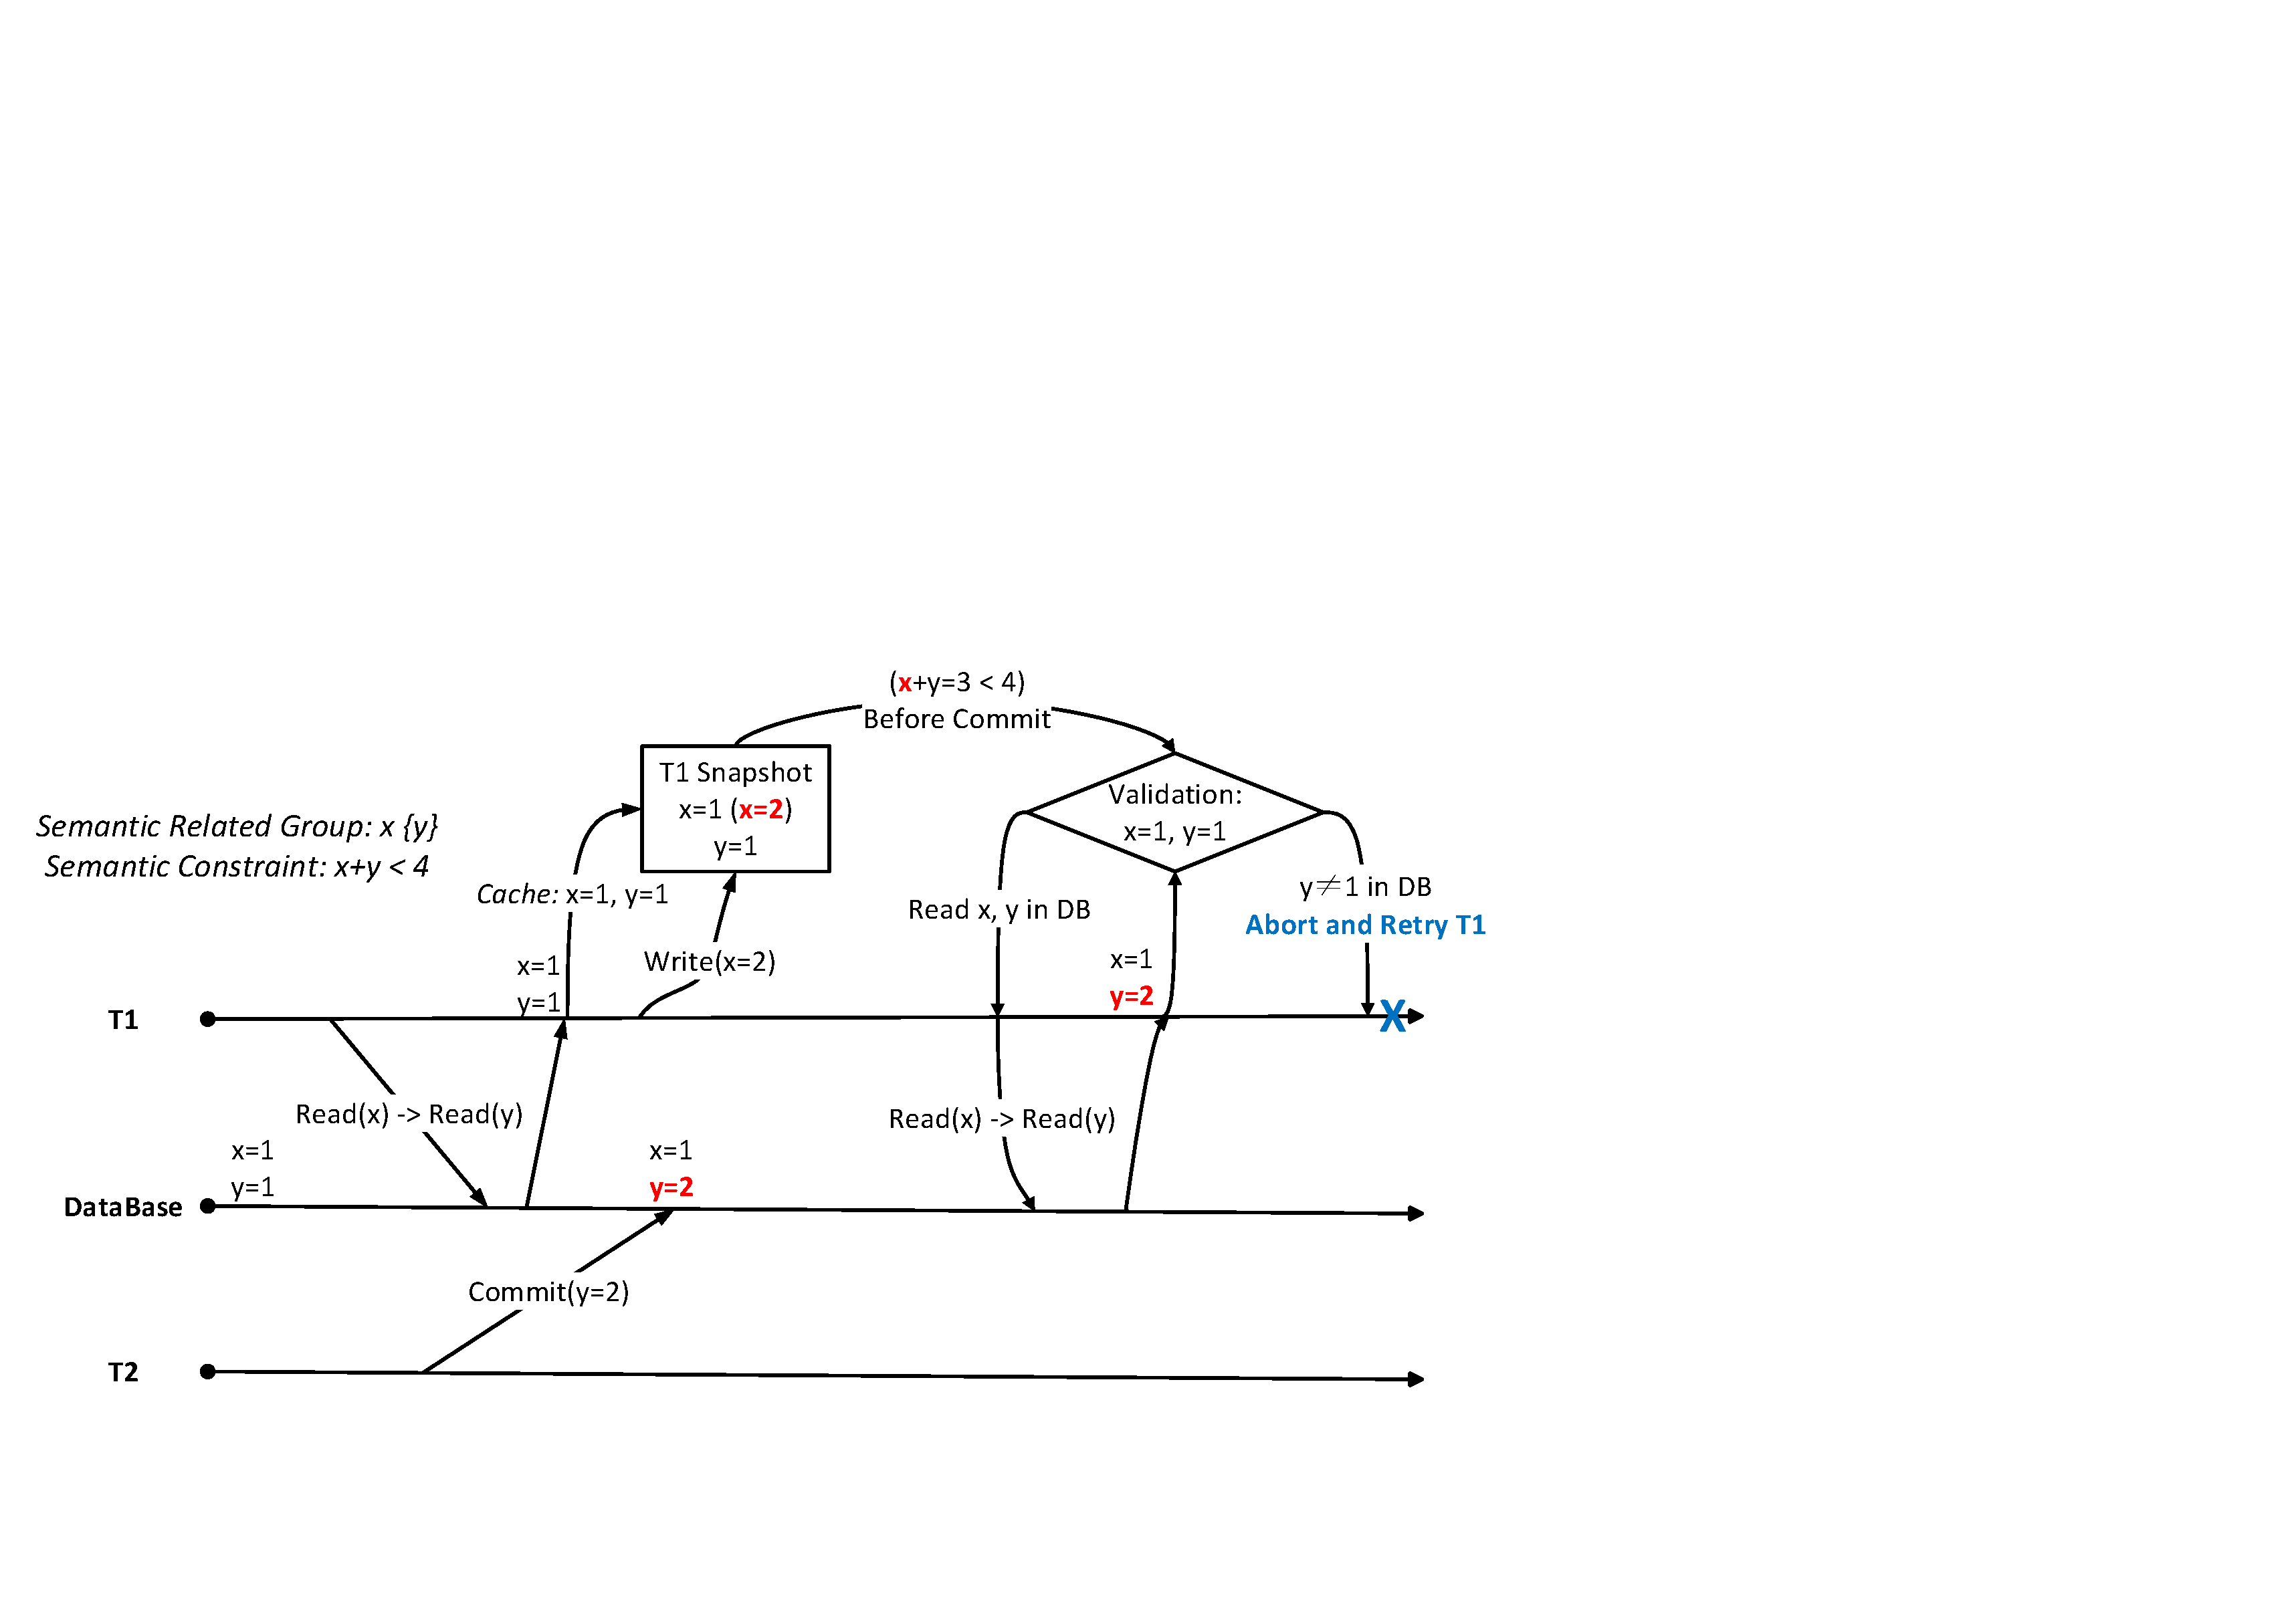
\includegraphics[width=\linewidth]{figs/snapwriteskew.pdf}
	\caption{Optimistic Concurrency Control with Snapshot Isolation on Semantic Related Group Precludes Write Skew}
	\label{fig:snapwriteskew}
\end{figure}

\noindent Therefore, we use optimistic concurrency control with snapshot isolation on semantic related group to improve the throughput while the strong consistency semantics in original HDFS is maintained.

\section{Total Order Update, Abort and Version Increase in Update Phase}
We have a total order update rule in update phase so that dead lock will not occur by lock cycle. If multiple rows needed to be during update phase, they will be sorted first by the \textit{id} value. Then they will be updated in ascending order according by \textit{ids}. 

\noindent Since we can not take an Exclusive lock on the "new" row which not yet exists in the database, multiple transactions may try to persist "new" rows with the same \textit{Primary Key}, and one might be overwritten by the other. Using \textit{makePersistent()} function in ClusterJ can throw exception if the instance already exists in the database.

\noindent Finally, for successful updates, the versions of the modified rows will be increased by 1.

\section{Pseudocode of the Complete Algorithm}

See Algorithm~\ref{algo:pseudocode}.
\begin{algorithm}[h]
	\caption{Pseudocode of the Complete Algorithm \\ Optimistic Concurrency Control with Snapshot Isolation on Semantic Related Group}
	\label{algo:pseudocode}
	\begin{algorithmic}[1]
		\STATE {\textbf{init:} restart = \TRUE, try = 0, path = operation.src, TotalRetry = 10}
		
		\WHILE{restart \AND try $<$ TotalRetry}
			\STATE {restart = \FALSE}
			\STATE {try += 1}
			\STATE {tx.snapshot.clear()}
			\STATE {tx.begin()}
			\STATE {\textit{\textbf{/* 1. Read Phase */}}}
			\STATE {tx.lockMode(\textit{Read\_Committed})}
			\STATE {tx.snapshot = resolve\_semantic\_related\_group(path)}
			\STATE {\textit{\textbf{/* 2. Execution Phase */}}}
			\STATE {operation\_performTask(tx.snapshot) // HDFS operation performs on its snapshot}
			\STATE {\textit{\textbf{/* 3. Validation Phase */}}}
			\STATE {tx.lockMode(\textit{Shared})}
			\STATE {relatedRows\_DataBase = batchRead\_Database(tx.snapshot)}
			\STATE {tx.lockMode(\textit{Exclusive})}
			\STATE {modifiedRows\_DataBase = batchRead\_Database(tx.snapshot)}
			\IF{versionCompare(relatedRows\_DataBase, tx.snapshot) $==$ \TRUE \textbf{ and} versionCompare(modifiedRows\_DataBase, tx.snapshot) $==$ \TRUE}
				\STATE {\textit{\textbf{/* 4. Update Phase */}}}
				\STATE {operation.modifiedRows.version+=1}
				\STATE {total\_order\_sort(operation.modifiedRows)}
				\IF{batchPersist\_Database(operation.modifiedRows) \textbf{success}}
					\STATE {tx.commit()}
					\STATE {return \textbf{SUCCESS} // Return HDFS Operation Success}
				\ELSE
					\STATE {tx.abort()} 
					\STATE{waitForRandomMilliseconds()}
					\STATE{retry = \TRUE}
				\ENDIF
			\ELSE 
				\STATE {tx.abort()}
				\STATE{waitForRandomMilliseconds()}
				\STATE{retry = \TRUE}
			\ENDIF
		\ENDWHILE
		
		\STATE {return \textbf{FAIL} // Return HDFS Operation} 
	\end{algorithmic}
\end{algorithm}

\section*{Summary}

In this chapter, we proposed a solution to improve the throughput in Hop-HDFS based optimistic concurrency control with snapshot isolation on semantic related Group. We gave all the details on related phases of the algorithm and discuss how anomalies are precluded in our solution. Finally, we provided the complete algorithm pseudocode for our solution.